\chapter{The cosmic microwave background}
\label{chp:cmb}

The cosmic microwave background (CMB) gives us our earliest view of the universe: most of the CMB photons we observe today last scattered about 380,000 years after the universe began, during a cosmological epoch called recombination.
Over the half century since the first detection, in 1965~\autocite{Penzias1965ApJ}, 
observations of the CMB have become increasingly precise and have informed much of our understanding of cosmology.
In this chapter I give an overview of CMB cosmology and CMB experiments in order to motivate the detector research described in later chapters.
Section~\ref{sec:cmb.physics} contains a brief history of the universe that focuses on the CMB and includes current experimental results.
In Section~\ref{sec:cmb.experiment}, I discuss the CMB from an experimental perspective: the goals of future experiments, the characteristics of measured signals, and the requirements for detectors.


\section{Physics}
\label{sec:cmb.physics}

\subsection{Before recombination}
\label{sec:cmb.physics.before}

The standard cosmological model, which contains a small number of free parameters and assumptions, is able to describe most astrophysical measurements~\autocite{Dodelson2003, Bartelmann2010RMP, Spergel2015Science}.
The available evidence supports a picture of a flat early universe that was very hot and dense, and was filled with a nearly homogeneous and isotropic soup of fundamental particles: the hot Big Bang.
Figure~\ref{fig:2015_SMICA_CMB} shows a recent measurement of the angular anisotropies of the CMB intensity (or temperature), which is an indirect picture of the primordial density perturbations.
As the CMB temperature today is about \SI{3}{K}, the peak fractional deviations are only about \num{e-4} and the root-mean-square deviations are an order of magnitude smaller.

\begin{figure}[tb]
\centering
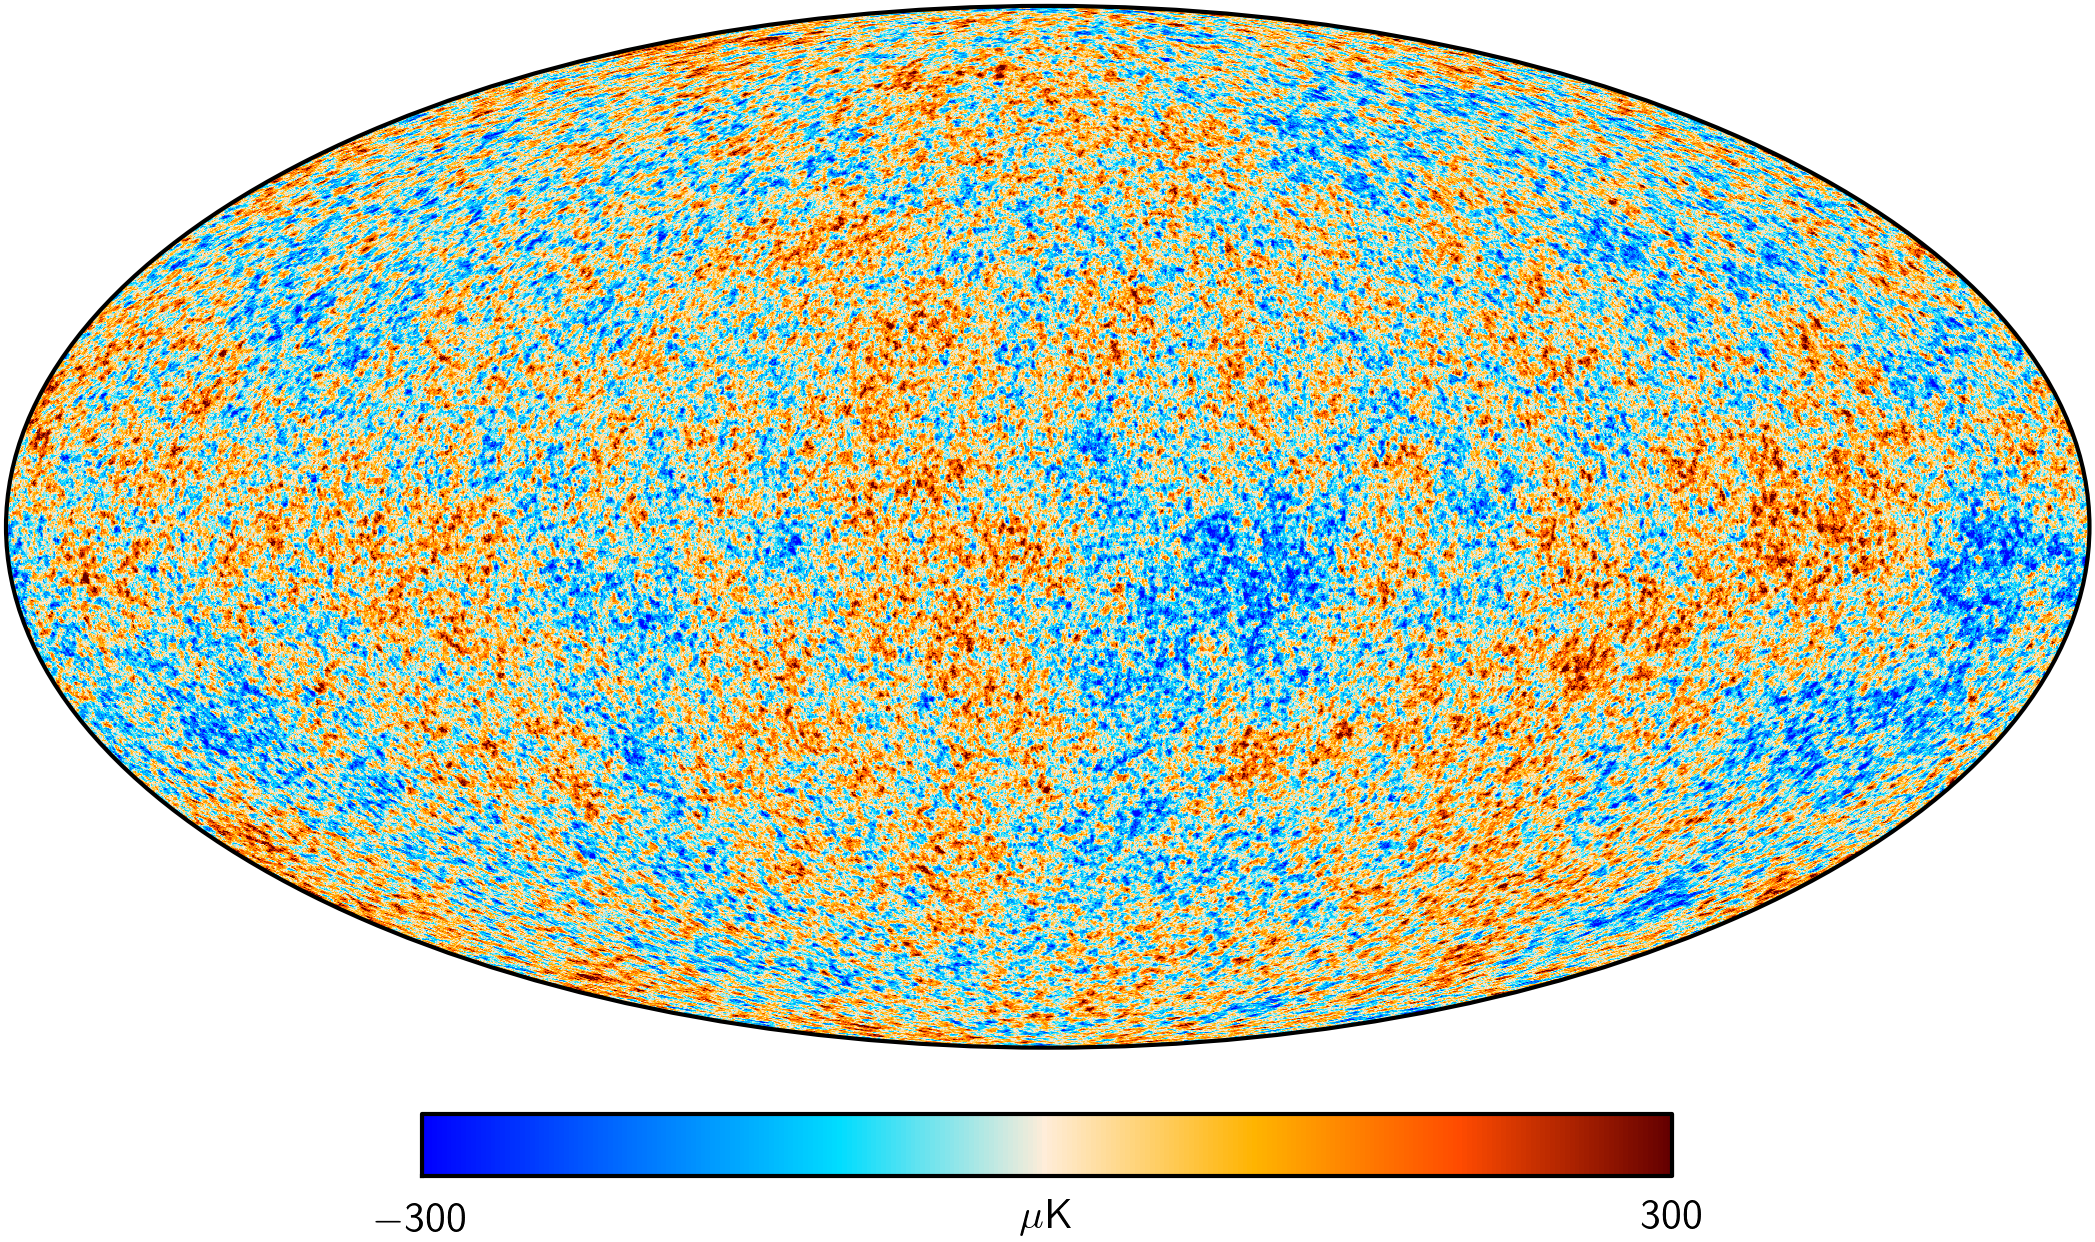
\includegraphics[width=\textwidth]{cmb/2015_SMICA_CMB.png}
\caption[A map of the CMB temperature anisotropies from the \textit{Planck} satellite.]
{
A map of the CMB temperature anisotropies using data from the \textit{Planck} satellite combined with other measurements~\autocite{Planck2015I}.
The color scale corresponds to the intensity deviations in units of temperature difference from the CMB mean temperature.
The angular resolution is 5'.
The CMB dipole due to our peculiar velocity has been removed, and galactic signals have been subtracted using observations at multiple frequencies, except for a small region in the galactic plane where the data has been generated randomly.
}
\label{fig:2015_SMICA_CMB}
\end{figure}

General relativity predicts the expansion rate of space, given its energy content.
On large scales, the expansion of a flat universe can be described by a single dimensionless parameter: the scale factor $a$.
The scale factor has increased monotonically over the history of the universe as we understand it, and is conventionally set to 1 today.
The evolution of the various components of the energy density depend in turn on the scale factor.
The energy density in matter goes as $\scalefactor^{-3}$, since the number of particles is conserved as the physical volume increases.
According to the standard model of cosmology, only 5\% of the current energy density of the universe is in the form of matter that is described by the standard model of particle physics.
An additional 25\% is in the form of cold dark matter that seems to not to interact electromagnetically.
Nearly all the remainder is in the form of dark energy, and observations are consistent with a cosmological constant that is independent of $a$.
The energy density in radiation, meaning photons and relativistic massive particles, goes as $\scalefactor^{-4}$; the additional factor of $\scalefactor$ arises from the cosmological redshift, or the stretching of each mode as space expands.
While radiation dominated the energy density of the early universe, it is negligible today.
The scale factor is closely related to the redshift
$\redshift
  =
  \wavelength_\mathrm{ob} / \wavelength_\mathrm{em} - 1
  =
  a^{-1} - 1$,
where $\wavelength_\mathrm{ob}$ and $\wavelength_\mathrm{em}$ are respectively the observed and emitted wavelengths of light.

Starting from the highest temperatures of which we have some experimental understanding, our observations support a picture of a universe that continually expands and cools while matter forms bound states of progressively lower energy and the components of radiation successively decouple.
The most widely studied models for even earlier times describe a period of nearly-instantaneous expansion called cosmic inflation~\autocite{Guth1981PRD}.
In order for such expansion to occur, inflationary models require adding one or more fields to the standard model of particle physics.
Since such fields are not observed today they must have decayed into more familiar fields at early times, and quantum fluctuations in the inflationary fields could have seeded the primordial density perturbations.
A generic prediction of inflation is a gravitational wave background that, if sufficiently large, would produce a characteristic imprint in the CMB.
Current experiments are searching for this imprint.

\begin{figure}[htb]
\centering
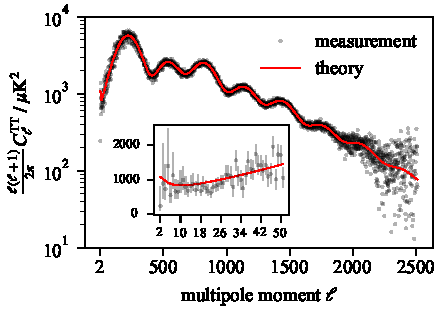
\includegraphics[width=\textwidth]{cmb/cmb_temperature_power_spectrum.pdf}
\caption[\textit{Planck} measurements of the CMB temperature power spectrum.]
{
\textit{Planck} measurements of the CMB temperature power spectrum.
The gray points are measured, unbinned, without error bars.
(One low outlier at high $\ell$ is not visible.)
The red curve is the prediction of the \textit{Planck} 2015 best-fit cosmology.
Measurements from ground-based experiments with larger primary apertures extend to much higher multipoles.
The inset shows the low-$\ell$ data on a linear scale, with error bars.
}
\label{fig:cmb_tt_power_spectrum}
\end{figure}

At very early times the temperature would have been too high for baryons to form, so this matter may have been in the form of the quark-gluon plasma that is studied through heavy-ion collisions in particle colliders~\autocite{Shuryak2017RMP}.
Around this time, some unknown process resulted in an excess of what we call matter over antimatter.
As the temperature decreased below that necessary for pair-production of baryons and anti-baryons, these mutually annihilated, leaving an excess of baryons.
When the temperature reached \SI{1}{MeV}, when the universe was about \SI{1}{s} old, the neutrinos decoupled.
Next, the electrons and positrons annihilated, leaving a universe that apparently contains no net charge and no antimatter.

By applying our understanding of nuclear physics to the conditions in the early universe, we can predict the relative abundances of  light nuclei, which would have formed when the temperature dropped to around \SI{0.1}{MeV}.
The predictions of this model of Big Bang nucleosynthesis agree well (except for $^7$Li) with current measurements of light elements corrected for processing in stars~\autocite{Cyburt2016RMP}.

\todo[inline]{Understand initial perturbation scales and their different evolution}
After the end of nucleosynthesis, the composition of the plasma did not change much until recombination began.
The initial perturbations were almost the same at all scales, but evolved differently.
In over-dense regions, increased gravitational attraction competed with increased radiation pressure from higher temperatures, and the plasma thus supported acoustic oscillations.
During this phase, when the temperature was of order \SI{10}{eV}, the energy density of radiation dropped below that of matter.


\subsection{During recombination}
\label{sec:cmb.physics.during}

Because of the large excess of photons over baryons, hydrogen did not form until the temperature had dropped to around \SI{0.25}{eV}, far below the hydrogen binding energy.
As recombination proceeded, over about 100,000 years, the universe became increasingly transparent.
Toward the end of recombination, the mean free path for photons became so large that they no longer scattered.
Perturbations in the primordial plasma were thus frozen in, and we observe them today in the CMB.
It turns out that the excess gravitational redshift for photons leaving over-dense regions outweighs the increased brightness due to the higher temperatures there, so colder regions observed today in the CMB correspond to hotter, higher density regions during recombination.

Cosmological models that assume isotropy and homogeneity can make only statistical predictions for fluctuations in the CMB.
Just as the spectral density is useful for characterizing time-stationary signals, the angular power spectrum of the CMB anisotropies is useful for comparing statistical predictions to measurements.
Since we measure the CMB on the celestial sphere, the angular power spectrum is computed using spherical harmonics characterized by the multipole moment $\ell$.
Power at a given $\ell$ corresponds to fluctuations at an angular scale of about $\SI{180}{\degree} / \ell$, which in turn corresponds to a length scale at recombination.
Figure~\ref{fig:cmb_tt_power_spectrum} shows the angular power spectrum of the CMB temperature anisotropies.
The first peak in the temperature power spectrum, at $\ell \sim 200$, or \SI{1}{\degree}, corresponds to the mode that reached its first maximum at recombination.
\todo[inline]{Understand acoustic peaks better}

\todo[inline]{CMB polarization fraction}
The CMB is also weakly linearly polarized, with the polarized intensity a few orders of magnitude more faint than the temperature anisotropies.
This linear polarization is produced by the density perturbations present during recombination: a quadrupole intensity perturbation oriented perpendicular to the line of sight produces net linear polarization along the line of sight due to elastic (Thomson) scattering.
The standard model predicts no circular polarization in the CMB, and measurements so far have produced only upper limits~\autocite{Nagy2017ApJ}.
The polarization of the CMB can thus be described by a pseudovector field on the celestial sphere.
Since there is no preferred orientation for the polarization field, it is useful to decompose it into an curl-free (even-parity) E-mode component and a divergence-free (odd-parity) B-mode component.
The density perturbations produce only E-mode polarization, which has been measured by many experiments.
The angular power spectrum of the E-modes measured by \textit{Planck} is shown in Figure~\ref{fig:cmb_polarization_power_spectrum}.

\begin{figure}[htb]
\centering
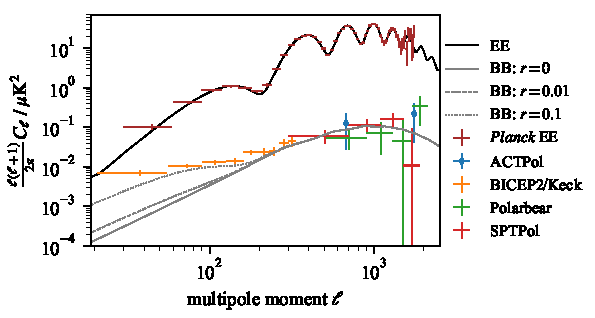
\includegraphics[width=\textwidth]{cmb/cmb_polarization_power_spectrum.pdf}
\caption[Recent measurements of the CMB E-mode and B-mode power spectra.]
{Recent measurements of the CMB E-mode and B-mode power spectra.
The E-mode data are from the 2015 \textit{Planck} release.
(Data at the lowest and highest multipoles, where the error bars are large, are not shown.)
The B-mode data were released by ACTPol~\autocite{ACTPol2017JCAP},
BICEP2/Keck Array~\autocite{BK2016PRL},
Polarbear~\autocite{Polarbear2017ApJ}, 
and SPTPol~\autocite{SPTPol2015ApJ}.
Data sets binned in other units have been converted to the displayed units using the center bin value, which is only approximately correct.
Where bins widths were available, these are shown by the horizontal bars; otherwise, a single point shows the center bin.
The theory curves were calculated with CAMB~\autocite{CAMB}: the solid black line and solid gray lines use the Planck 2015 best-fit cosmology~\autocite{Planck2015XIII}, and the dashed and dotted gray lines also include a nonzero tensor-to-scalar ratio $r$.}
\label{fig:cmb_polarization_power_spectrum}
\end{figure}

Gravitational waves decay as the universe expands, and any that were produced by inflation would be undetectable today.
However, gravitational waves present during recombination would have imprinted a primordial B-mode signature in the CMB.
\todo[inline]{Understand exact definitions of $r$}
The amplitude of these perturbations is commonly modeled by adding one parameter, the tensor-to-scalar ratio $r$, to the standard model.
Figure~\ref{fig:cmb_polarization_power_spectrum} shows the angular power spectrum of the B-modes measured by recent experiments as well as theoretical predictions for several values of $r$.
Larger values of $r$ correspond to larger signals in the B-mode power spectrum, and this primordial signal could be measurable at large angular scales.
However, the amplitude of the inflationary signal is not well-constrained by theory, and could be too small to measure even if inflation occurred.
The data points from the BICEP2 and Keck Array experiments show an excess B-mode signal at low multipoles, but this signal is dominated by galactic dust~\autocite{BKP2015PRL}.
The current upper limit from CMB data is $r < 0.09$ at 95\% confidence~\autocite{BK2016PRL}.


\subsection{After recombination}
\label{sec:cmb.physics.after}

After recombination, the baryons are almost entirely in the form of neutral hydrogen and helium.
The CMB photons thus pass freely through the universe as the over-dense regions slowly collapse into the structure we see today.
Although the CMB no longer exchanges much energy with matter, the gravitational redshift turns out to preserve the shape of the black body curve, and the CMB remains a nearly-perfect black body at a temperature inversely proportional to the scale factor.

Today, the CMB temperature is reduced by a factor of the redshift at recombination, approximately 1100, to $\temperature_\mathrm{CMB} = \SI{2.7255}{K} \pm \SI{0.0006}{K}$~\autocite{Fixsen2009ApJ}.
Figure~\ref{fig:firas_monopole_spectrum} shows the spectrum of the CMB measured by the FIRAS instrument on the COBE satellite.
For a black body at the CMB temperature the peak of the brightness spectral density occurs near frequency $\foptical = \SI{160}{GHz}$, and the occupancy
$\photonoccupancy(\foptical) = [\exp(\planck \foptical / \kb \temperature_\mathrm{CMB}) - 1]^{-1}$ drops below 1 above $\foptical \approx \SI{40}{GHz}$.

\begin{figure}[tb]
\centering
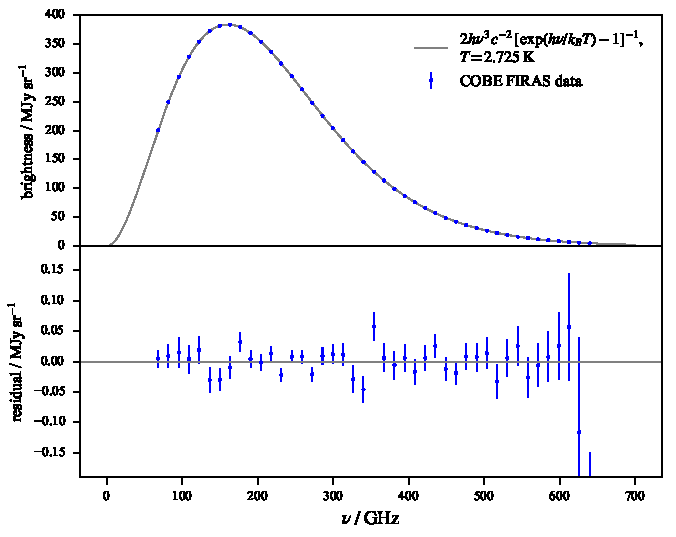
\includegraphics[width=\textwidth]{cmb/firas_monopole_spectrum.pdf}
\caption[The CMB monopole spectrum from FIRAS on COBE.]
{
The CMB monopole spectrum from the FIRAS instrument on the COBE satellite~\autocite{Fixsen1996ApJ, Fixsen2002ApJ}.
\textbf{(Upper)} The blue points are measured (with error bars that are too small to be visible), and the gray line is the black body curve given in the legend.
\textbf{(Lower)} Residuals from the upper panel.
The blue points are the measured data minus the model.
}
\label{fig:firas_monopole_spectrum}
\end{figure}

The CMB we detect today originates from a distant last-scattering surface, and it has been altered during the subsequent history of the universe.
CMB photons do not interact much during the so-called cosmic dark ages, until the first stars form and begin to emit photons that have sufficient energy to reionize the neutral gases.
\todo[inline]{Redshift of reionization.}
However, even after reionization, only a small fraction of CMB photons scatter.
\todo[inline]{Effect of reionization on the CMB.}
Weak gravitational lensing converts E-mode polarization into B-mode polarization at an amplitude that can be calculated from the known evolution of the matter distribution since recombination. 
In Figure~\ref{fig:cmb_polarization_power_spectrum}, the B-mode measurements at smaller angular scales are roughly consistent with the expected amplitude due to lensing.

\todo[inline]{Incorporate material on LCDM parameters.}
\begin{comment}
\subsection{The standard model of cosmology}
\label{sec:cmb.physics.cosmology}

Most of the parameters of the standard model of cosmology relate to fundamental gaps in our understanding.
The age of the universe and the spectral index of primordial fluctuations describe a universe that has a finite age and began in a hot, dense, and slightly inhomogeneous state.
The spectral index quantifies the amplitude of these primordial fluctuations in the density and temperature as a function of their size initial, but the mechanism that seeded these initial conditions is uncertain.
Two parameters describe the fractional energy content of the universe in baryons (the cosmological term that encompasses all hadron and lepton matter) and in cold dark matter (CDM), which are respectively about 5\% and 25\% of the total.
Measurements on widely-differing scales provide strong evidence for a particle that does not interact electromagnetically, but such a particle is not described by the standard model of particle physics and has not been directly detected.
Even the prosaic baryon fraction relates to the mystery of the excess of matter over antimatter that presumably produced the initial matter and photon content through annihilation.
The remaining energy content, about 70\% of the total, is apparently in the form of dark energy, modeled as a cosmological constant $\Lambda$, which causes the accelerating expansion of the universe.
One parameter relates to the curvature of the universe on large scales: current measurements are consistent with the universe being flat, but there is no known reason for this to be the case.
The final parameter, the optical depth to reionization, simply describes the opacity of the universe to CMB photons.
Fortunately, even the recent universe is fairly transparent, which has allowed us to learn much of what we know about cosmology.
\end{comment}


\section{Experiment}
\label{sec:cmb.experiment}

\subsection{Goals}
\label{cmb.experiment.goals}

Current CMB mapping experiments focus on polarization in order to improve on the measurements shown in Figure~\ref{fig:cmb_polarization_power_spectrum}.
A major goal is to search for the signature of primordial B-modes produced by inflation, which would give valuable information about physics at higher energies than we can currently probe.
\todo[inline]{Understand neutrino mass constraints}
Another major experimental goal is to constrain the sum of the masses of all neutrino species, which is possible because all of the constituents of the primordial plasma affect the CMB~\autocite{CMBS4ScienceBook}.
By contrast, neutrino oscillation experiments are sensitive to differences in the squares of the neutrino masses.

Since the CMB photons traverse nearly the entire visible universe, signals from closer sources are called foregrounds.
Polarized galactic foregrounds are brighter than the CMB polarization at most frequencies, and this is a major experimental challenge.
Overcoming it requires measurements in different frequency bands around the CMB peak in order to model and subtract the foreground signals.
The multichroic pixels described in Chapter~\ref{chp:multichroic} can each simultaneously measure two linear polarization states in two spectral bands.


\subsection{Signals}
\label{sec:cmb.experiment.signals}

In a typical band containing the \SI{160}{GHz} peak of the CMB spectrum, a detector on a space-based instrument with very cold optics would absorb about \SI{0.1}{pW}, or \SI{e9}{photons/s}.
The load in a ground-based instrument might be three orders of magnitude greater because the atmosphere is emissive in the millimeter-wave region and is much hotter than the CMB.
In both cases, the time between photon arrivals is much less than the response time of the detector, which thus measures only the average photon flux.

The fractional anisotropies of the CMB intensity are of order \num{e-5}, so the linearity and dynamic range requirements will be set by other, larger signals.
Experiments may observe bright calibrators, such as planets or artificial linearly polarized sources used to measure detector polarization angles.
Ground-based experiments must also contend with atmospheric fluctuations: even at the dry, high-altitude sites that are used for ground-based CMB observations, the atmosphere is much brighter than the CMB, with a typical effective Rayleigh-Jeans temperature of several tens of kelvin.

In principle, a CMB telescope could point at a particular location on the sky, average down the noise to the desired level, then move to another location.
In practice, this is not done because slow drifts in the instrument response produce systematic effects that are difficult to correct. 
Thus, a telescope typically scans repeatedly over the same 
patch of sky and revisits any given point many times.
(For polarimetry, it is useful to scan the same point on the sky from different instrument orientations, as this tends to average down some systematic errors.)
To reduce the demands on detector linearity, ground-based instruments often perform such scans at a constant elevation to maintain a constant load from the atmosphere.

Beams in existing instruments are designed to be approximately Gaussian with an angular diameter from about \SI{1}{\arcminute}~\autocite{ACT2011ApJS} to \SI{30}{\arcminute}~\autocite{BICEP2II2014ApJ},
typically limited by diffraction at the primary aperture.
The beam acts as a filter: information on scales much smaller then the beam is averaged out.
As a detector scans across the sky, modes at different angular scales are modulated at different frequencies in the time-ordered data.
A mode with angular wavelength $\lambda$ will appear in the time-ordered data of a detector scanning the sky with angular velocity $\dot{\theta}$ at audio frequency
$\faudio = \dot{\theta} / \lambda$, and the beam will create a low-pass filter in the frequency domain.
To avoid the difficulty of deconvolving the detector response from the time-ordered data, the detector bandwidth should be significantly greater than the bandwidth of this filter.

CMB polarimeters may use a modulator to separate the intensity signal from the fainter polarization signal in the frequency domain.
For example, a spinning half-wave plate will cause a constant polarization signal to appear in a power detector, or ``square-law'' detector, at four times its rotation frequency.
Modulation of the polarization at \SI{10}{Hz} has been demonstrated to work in a ground-based experiment~\autocite{Kusaka2014RSI},
and a prototype superconducting bearing system exists that could modulate at \SI{40}{Hz} or more~\autocite{Johnson2017RSI}.
The spectral density of detector data is typically red below a ``knee'' frequency at \SIrange{0.1}{10}{Hz} due to fluctuations in the atmospheric signal or in the detector system itself.
Thus, modulation may shift the polarization signal to a frequency band where the data is less contaminated by red noise.

The CMB anisotropies of current interest are faint in the sense that significant time may be needed to measure them, even when the only noise is due to the randomness of photon arrival times.
Existing detectors have sensitivity near this photon-noise limit, even in space, where the CMB may be the main contribution to the total detected power.


\subsection{Detectors}
\label{sec:cmb.experiment.detectors}

We can extract criteria for CMB detectors from the preceding discussion.
The detectors must be sufficiently linear to not distort the measured signals; the exact requirement will depend on the calibration strategy, and nonlinearity may be mitigated by injecting calibration signals.
The ideal noise level is less than the photon noise under the expected optical load, which depends on the instrument design and location.
The detector noise requirements are progressively more stringent for ground-based, balloon-borne, and space-based instruments.
The detector bandwidth should be sufficiently large to accommodate all signals of interest without excessive distortion.
For an instrument without polarization modulation that scans slowly, a bandwidth of \SI{10}{Hz} or less might be sufficient.
Using either a continuous calibration signal or a fast polarization modulator might increase the bandwidth requirement by an order of magnitude.

The detector technologies that have shown competitive sensitivity for CMB experiments all operate at temperatures below about \SI{1}{K}.
For the cryogenic requirements, and thus the cost, to be manageable, it must be possible to read out many of these cryogenic detectors using a small number of wires.
Techniques in use include time-division multiplexing, in which many detectors on a common wire are interrogated sequentially using switches, and frequency-division multiplexing, in which many detectors on a common wire are interrogated simultaneously using signals at unique frequencies that are somehow filtered so that each signal interacts with only one detector.

When the noise added by a detector is less than the photon noise, the only way to significantly increase the mapping speed of a detector array is to increase the number of detectors.
Most current suborbital experiments use transition-edge sensor (TES) bolometers.
The motivation for the work done in this thesis is that the kinetic inductance detector (KID), which naturally lends itself to frequency multiplexing, may offer an easier route to deploying larger arrays.
Current ground-based experiments use thousands of detectors, and proposed experiments will use tens or hundreds of thousands of detectors~\autocite{CMBS4TechnologyBook}.

